\documentclass[12pt,a4paper]{article}
\usepackage[UTF8]{ctex}
\usepackage{amsmath}
\usepackage{graphicx}
\usepackage{booktabs}
\usepackage{geometry}
\usepackage{siunitx}
\usepackage{ulem}
\usepackage{caption}
\usepackage{subcaption}
\geometry{left=2.5cm,right=2.5cm,top=2.5cm,bottom=2.5cm}
\sisetup{per-mode=symbol}
\graphicspath{{assets/}{5.25/}{processed/}}

\title{\Huge{\textbf{\uuline{实\ 验\ 报\ 告}}}}
\author{\uline{少年班学院} \quad 姓名: \uline{李大恕} \quad 学号: \uline{PB24000145}}
\date{2026年5月26日}

\begin{document}
\maketitle

\section{实验题目}
部分相干光源的空间相干性测量与分析

\section{实验目的}
\begin{enumerate}
    \item 理解部分相干光源的空间相干性及其随横向距离衰减的物理含义。
    \item 掌握利用激光与旋转毛玻璃产生部分相干光的方法。
    \item 熟悉改进迈克尔逊干涉光路中光程差、平面镜倾角和柱透镜反转对干涉图样的影响。
    \item 观察不同毛玻璃状态和位置下干涉条纹区域及条纹对比度的变化，分析部分相干光的空间相干特性。
\end{enumerate}

\section{实验原理}
\subsection{部分相干光的空间相干性}
部分相干光的重要特征是光场中不同横向位置之间只具有有限的相干性。两点之间的横向距离越大，其相干程度越弱，因而只有距离较近的光场点之间才能形成较清晰、稳定的干涉条纹。以部分相干的 Collett-Wolf 光源为例，空间相干度 $g(\rho)$ 与两点间距离 $\rho$ 的关系可写为
\begin{equation}
    g(\rho)=\exp\left(-\frac{\rho^2}{2\sigma_g^2}\right),
    \label{eq:coherence}
\end{equation}
其中 $\sigma_g$ 是相干性衰减的特征尺度。当 $\rho$ 超过这一尺度后，相干度迅速减小，干涉条纹的可见度也随之下降。

部分相干光在远距离传输过程中光强分布较为均匀，干涉条纹清晰稳定，同时可以有效降低激光散斑的影响；但其空间相干性会随横向距离快速衰减，因此横向相距较远的两束光难以产生明显干涉。

\subsection{迈克尔逊干涉与条纹对比度}
在迈克尔逊干涉仪中，入射光经分束后形成两束光，两束光分别经平面镜反射后重新叠加。调节两臂的光程差可以改变干涉相位，调节平面镜之间的相对倾角可以得到不同方向和不同间距的干涉条纹。

干涉条纹的清晰程度通常用条纹对比度表示：
\begin{equation}
    V=\frac{I_{\max}-I_{\min}}{I_{\max}+I_{\min}},
    \label{eq:visibility}
\end{equation}
其中 $I_{\max}$ 和 $I_{\min}$ 分别为局部条纹强度的最大值和最小值。对于部分相干光，条纹对比度与两束叠加光之间的相干程度密切相关。当两束光对应的源面点横向间距较小时，互相干性较强，条纹对比度较高；当对应点间距增大时，互相干性降低，条纹逐渐变浅甚至消失。

\subsection{部分相干光源相干性测量光路}
实验在迈克尔逊干涉光路的基础上进行改造，用激光与旋转毛玻璃组合产生部分相干光源，并在其中一路加入柱透镜，使分束后的某一束光在竖直方向发生反转。实验光路如图~\ref{fig:optical_path} 所示。

\begin{figure}[htbp]
    \centering
    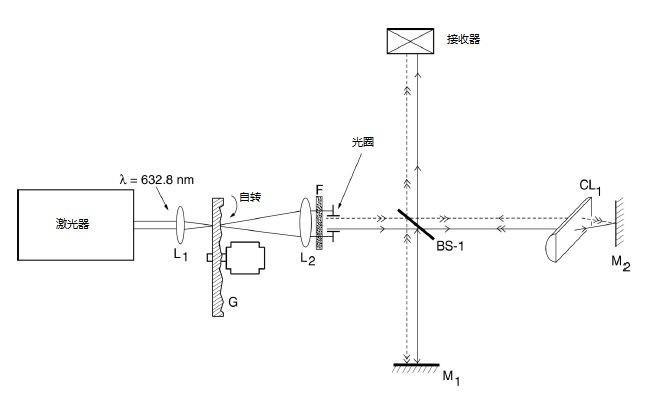
\includegraphics[width=0.72\textwidth]{page2_img2_Image53.jpg}
    \caption{部分相干光空间相干性测量光路}
    \label{fig:optical_path}
\end{figure}

激光经透镜扩束和毛玻璃散射后形成具有有限空间相干尺度的光场，再经光阑、分束器和平面镜构成双光束干涉。由于柱透镜将其中一路光束作竖直方向反转，屏幕或 CCD 上同一位置处叠加的两束光实际对应于源面上一对互为镜像的光场点。两点之间的横向距离随观察位置改变而改变，因此不同区域的条纹对比度不同。靠近相干性较好的重合区域时，条纹较清晰；远离该区域时，两束光对应点的横向间距增大，空间相干性减弱，条纹逐渐消失。

\section{实验仪器}
实验装置如图~\ref{fig:device} 所示，主要元件包括：
\begin{itemize}
    \item 波长为 \SI{532}{\nano\meter} 的半导体激光器；
    \item 焦距为 \SI{15}{\milli\meter} 的凸透镜 L1；
    \item 焦距为 \SI{50}{\milli\meter} 的凸透镜 L2；
    \item 毛玻璃 G 及其步进电机；
    \item 直径可调的光阑 F；
    \item 平面镜 M1、M2；
    \item 焦距为 \SI{2}{\centi\meter} 的水平放置柱透镜 CL1；
    \item 分束器、CCD 成像系统及光学平台。
\end{itemize}

\begin{figure}[htbp]
    \centering
    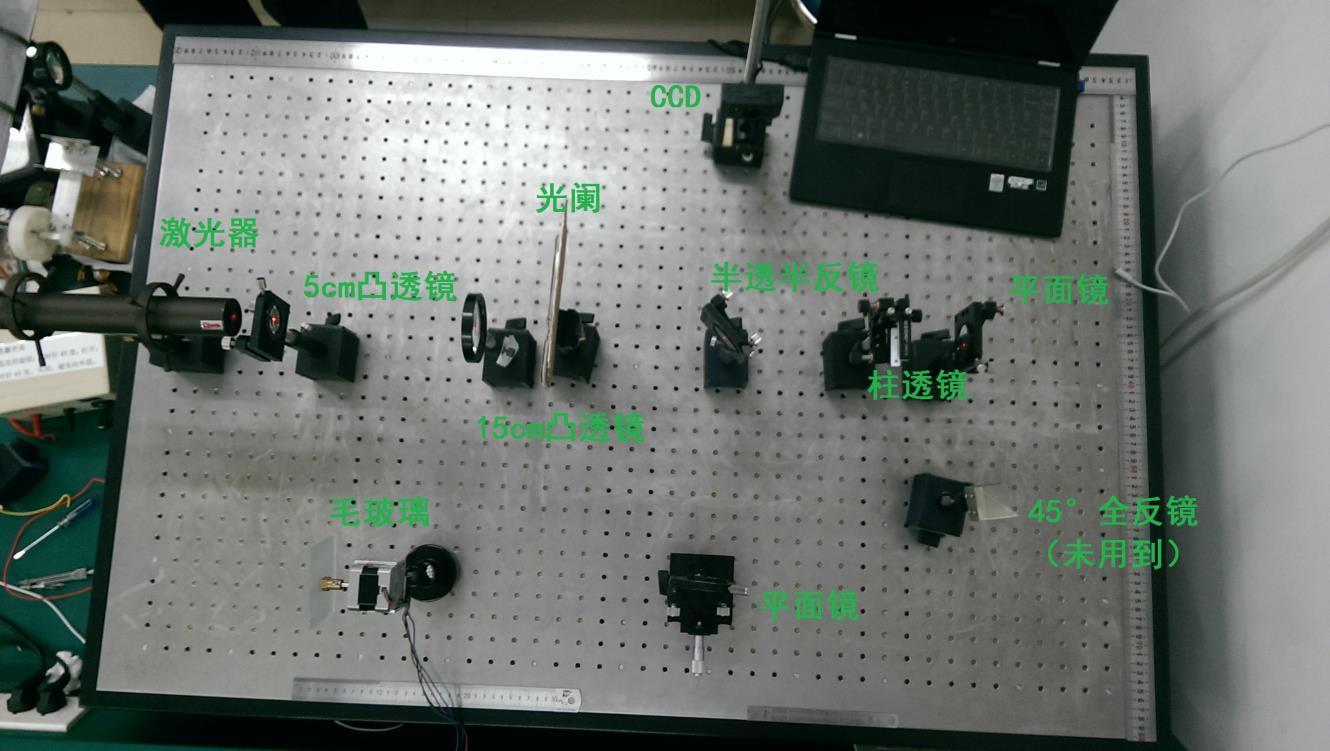
\includegraphics[width=0.82\textwidth]{page3_img1_Image63.jpg}
    \caption{部分相干光空间相干性测量实验装置}
    \label{fig:device}
\end{figure}

\section{实验过程}
\begin{enumerate}
    \item 按实验光路安装激光器、透镜、毛玻璃及步进电机、光阑、分束器、平面镜、柱透镜和 CCD，使各光学元件共轴，光轴平行于光学平台。
    \item 调整下方平面镜的位置和倾角，使 CCD 图像上的干涉条纹尽可能粗。此时两分光路近似等光程，两平面镜近似互相垂直。
    \item 继续微调平面镜，使两平面镜在水平或竖直方向存在适当夹角，分别获得竖直、水平或倾斜方向的干涉条纹，并观察条纹间距的变化。
    \item 在未加入毛玻璃的条件下观察普通迈克尔逊干涉图样，记录条纹方向、间距和清晰程度。
    \item 加入静止毛玻璃，观察散斑背景中的干涉条纹，比较其与未加入毛玻璃时的差别。
    \item 启动步进电机使毛玻璃旋转，观察条纹范围和对比度的变化。重点记录条纹是否只在部分区域保留，以及中间区域和两侧区域的条纹清晰程度。
    \item 改变旋转毛玻璃的位置，记录存在明显干涉条纹的区域变化。
\end{enumerate}

\section{实验现象与图像记录}
实验所得 CCD 图像保存在 \texttt{5.25} 文件夹中。为便于在报告中引用，原始 BMP 图像已转换为 PNG 图像，图像内容未作物理量修正。实验图像记录如图~\ref{fig:records1} 和图~\ref{fig:records2} 所示。

\begin{figure}[htbp]
    \centering
    \begin{minipage}{0.31\textwidth}
        \centering
        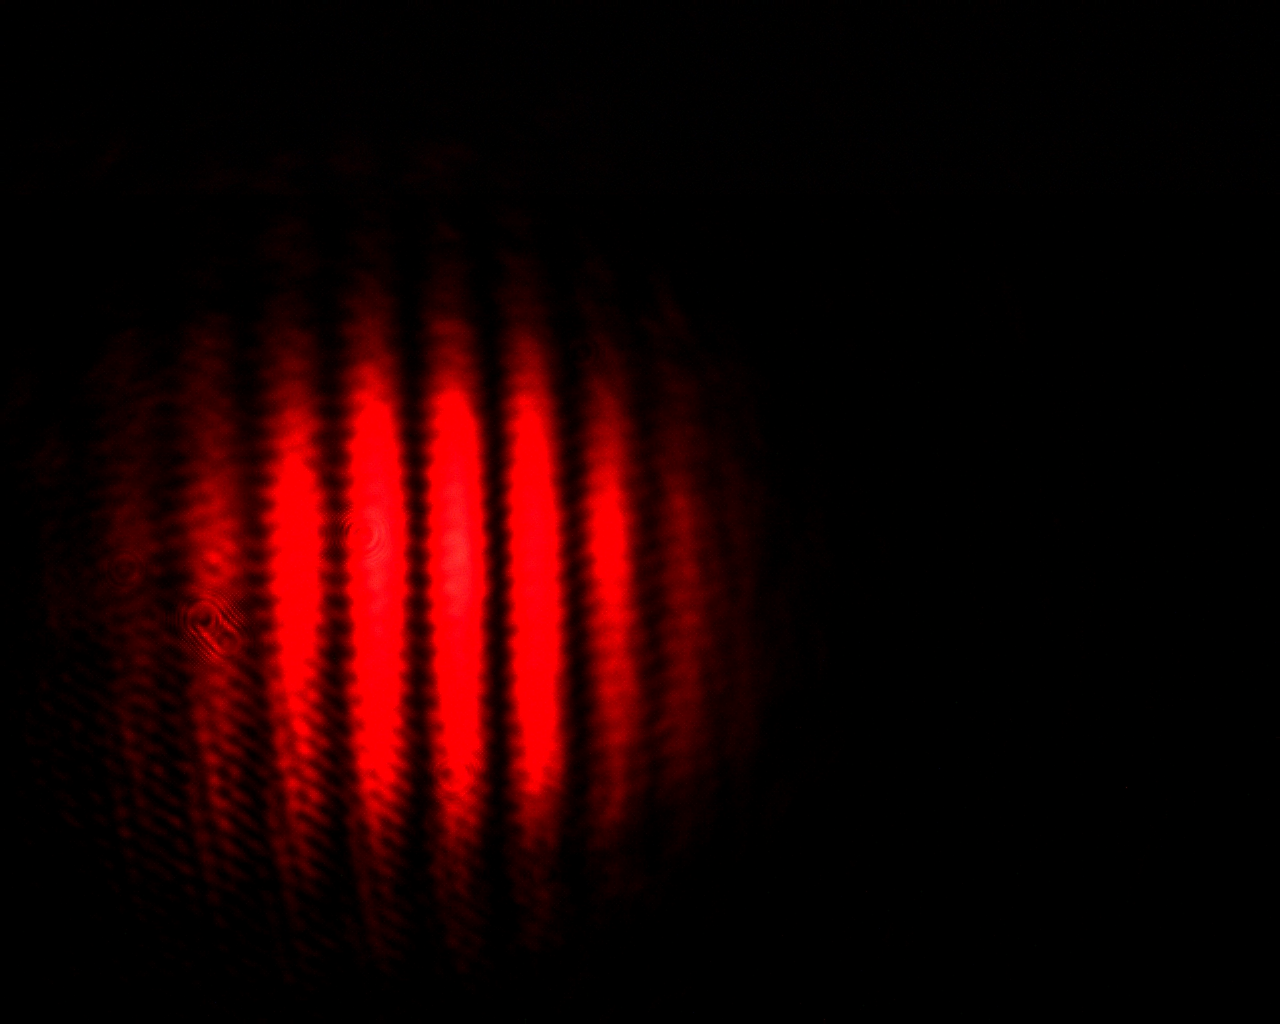
\includegraphics[width=\textwidth]{Pic_20260525192628038.png}
        \caption*{(a)}
    \end{minipage}
    \hfill
    \begin{minipage}{0.31\textwidth}
        \centering
        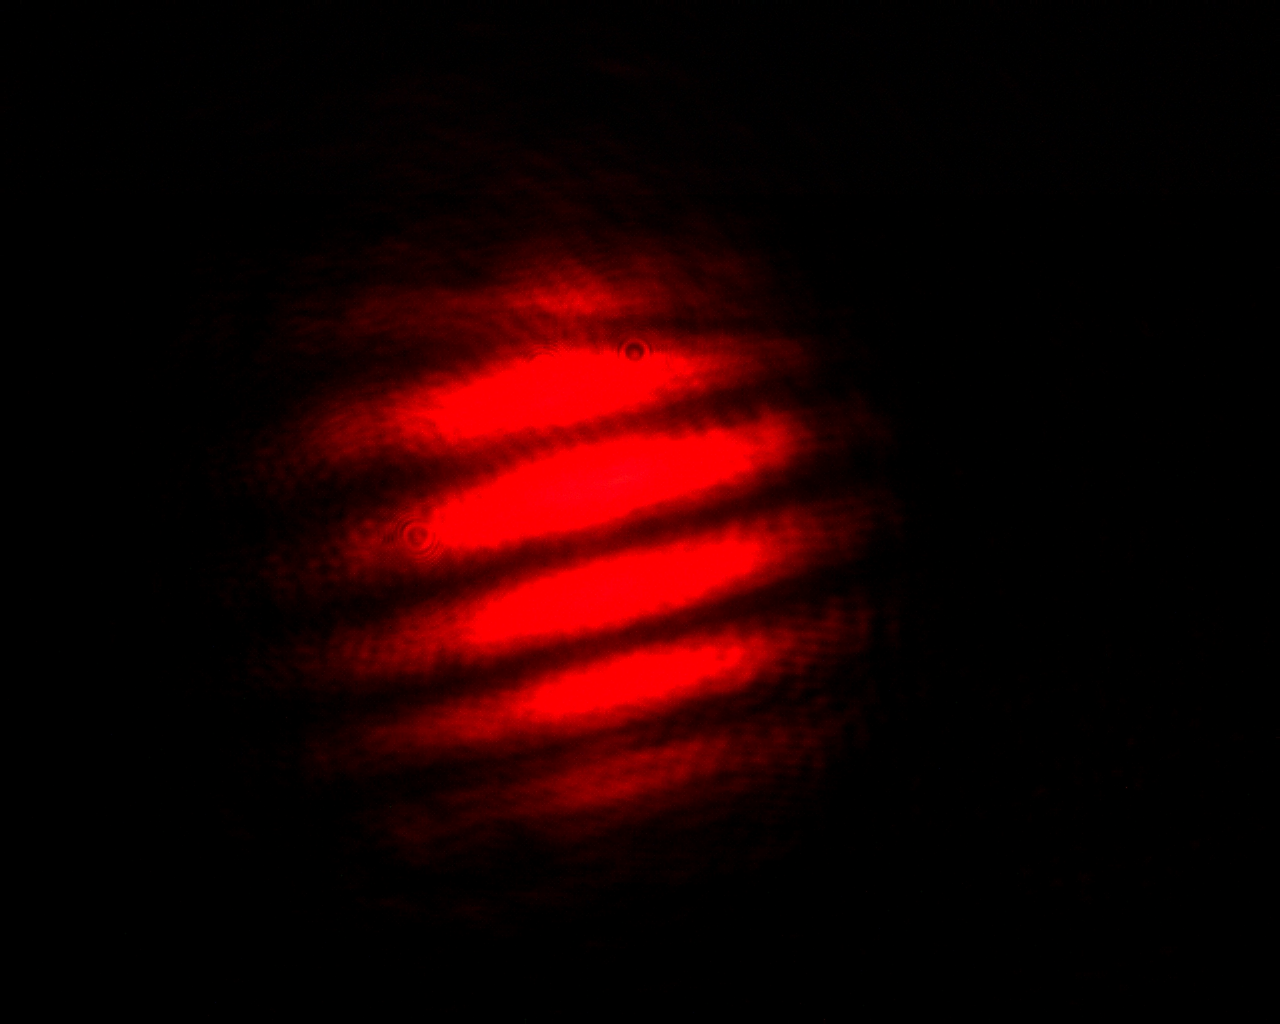
\includegraphics[width=\textwidth]{Pic_20260525194646918.png}
        \caption*{(b)}
    \end{minipage}
    \hfill
    \begin{minipage}{0.31\textwidth}
        \centering
        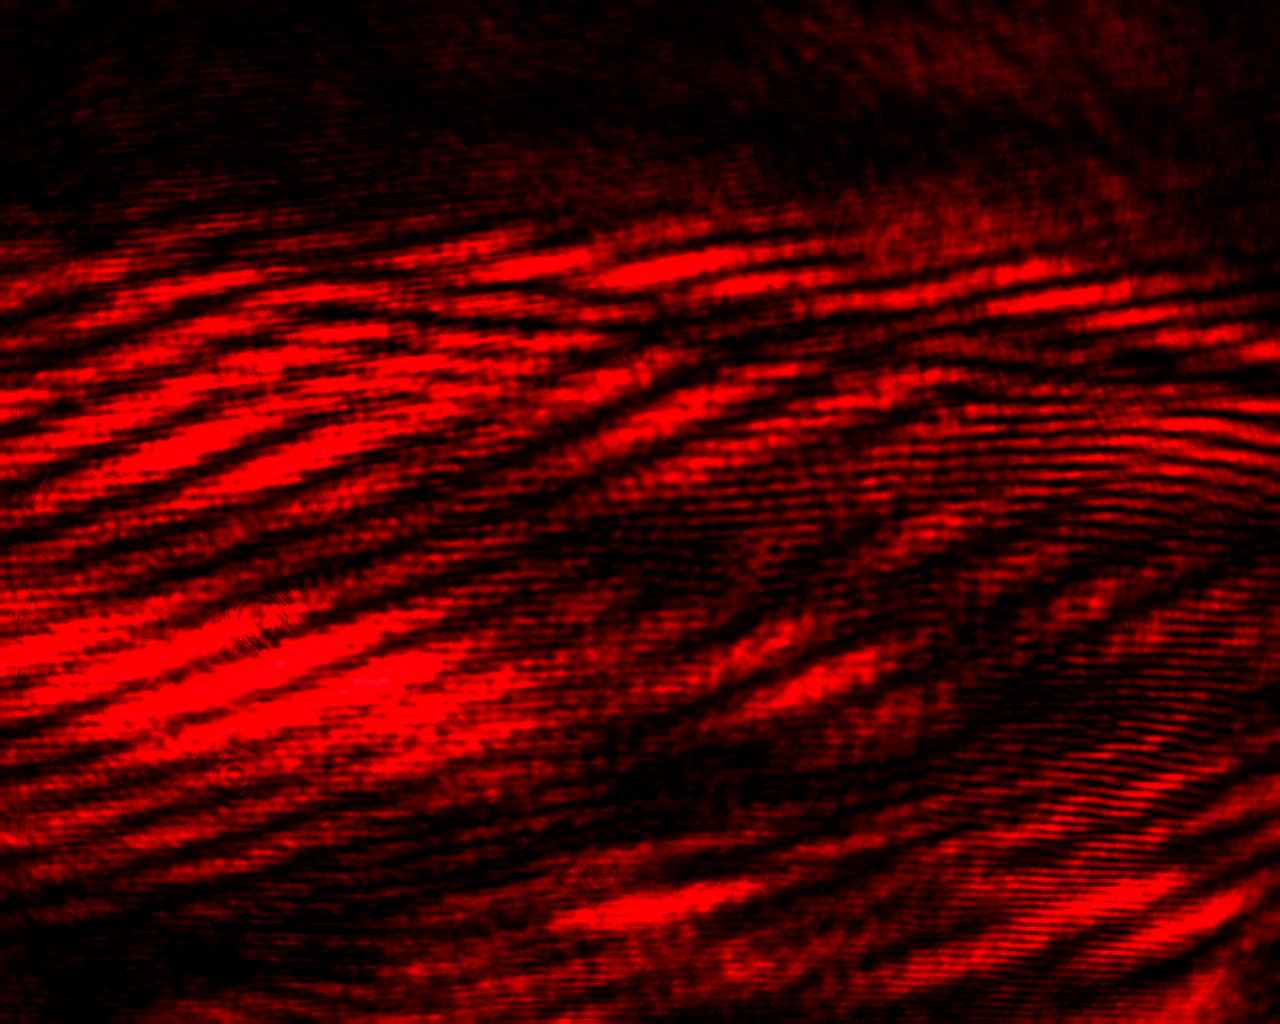
\includegraphics[width=\textwidth]{Pic_20260525195435698.png}
        \caption*{(c)}
    \end{minipage}
    \caption{实验记录图像（一）}
    \label{fig:records1}
\end{figure}

\begin{figure}[htbp]
    \centering
    \begin{minipage}{0.31\textwidth}
        \centering
        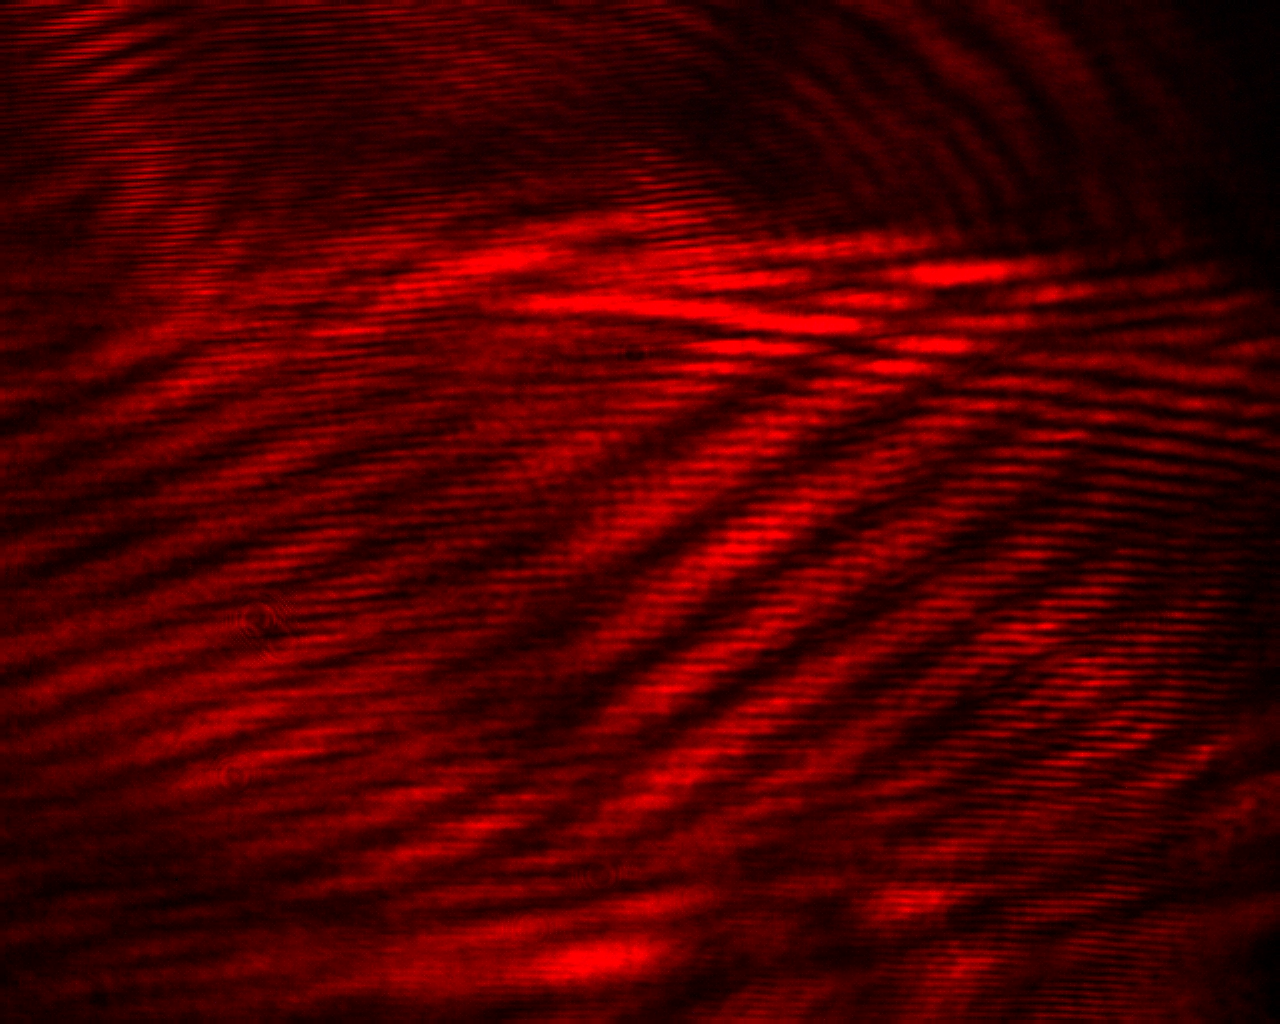
\includegraphics[width=\textwidth]{Pic_20260525195448209.png}
        \caption*{(d)}
    \end{minipage}
    \hfill
    \begin{minipage}{0.31\textwidth}
        \centering
        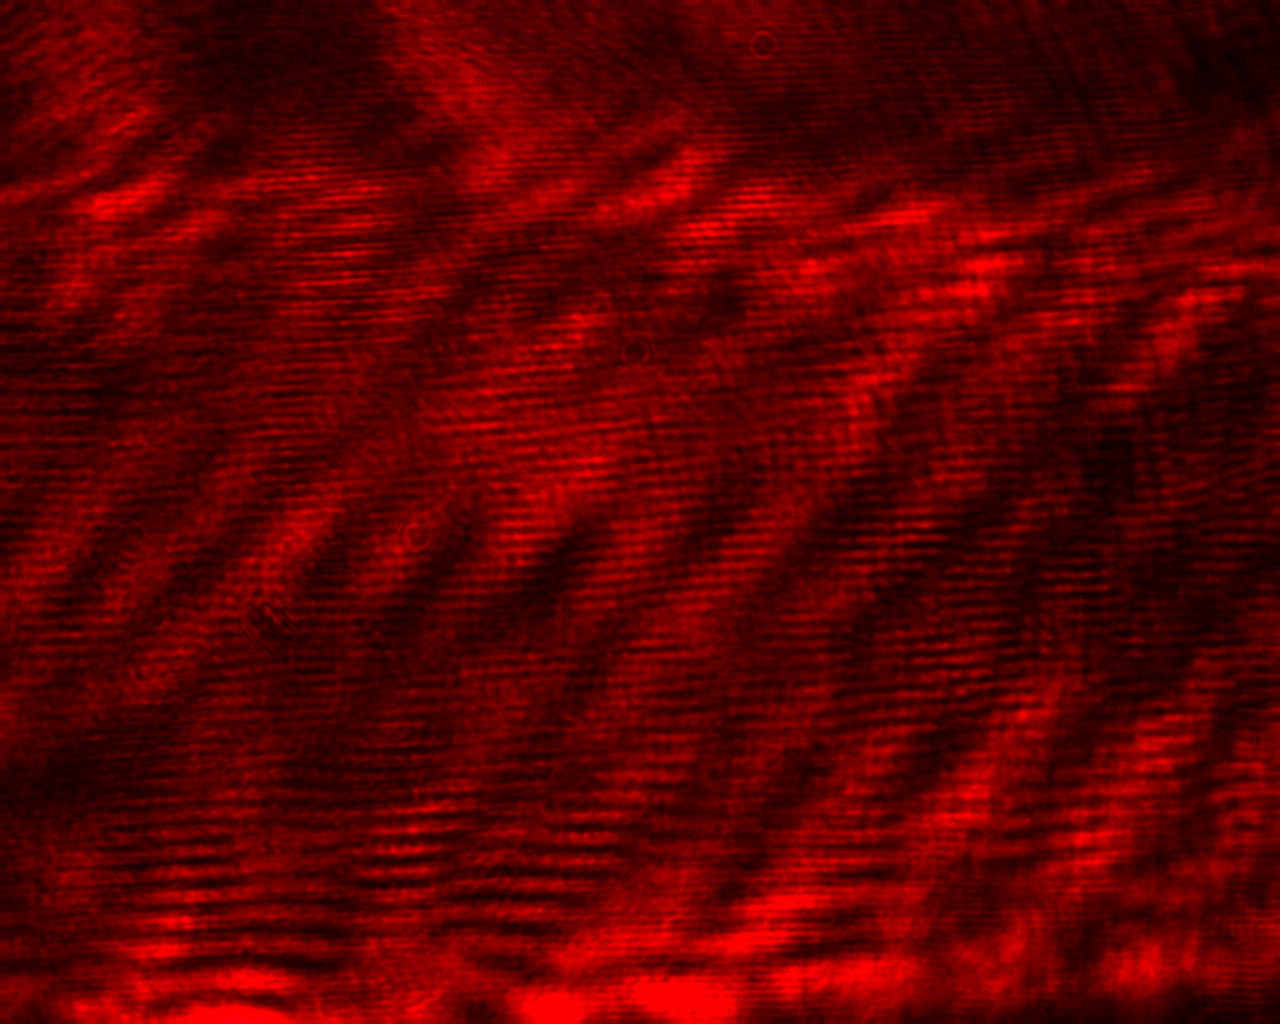
\includegraphics[width=\textwidth]{Pic_20260525203147728.png}
        \caption*{(e)}
    \end{minipage}
    \hfill
    \begin{minipage}{0.31\textwidth}
        \centering
        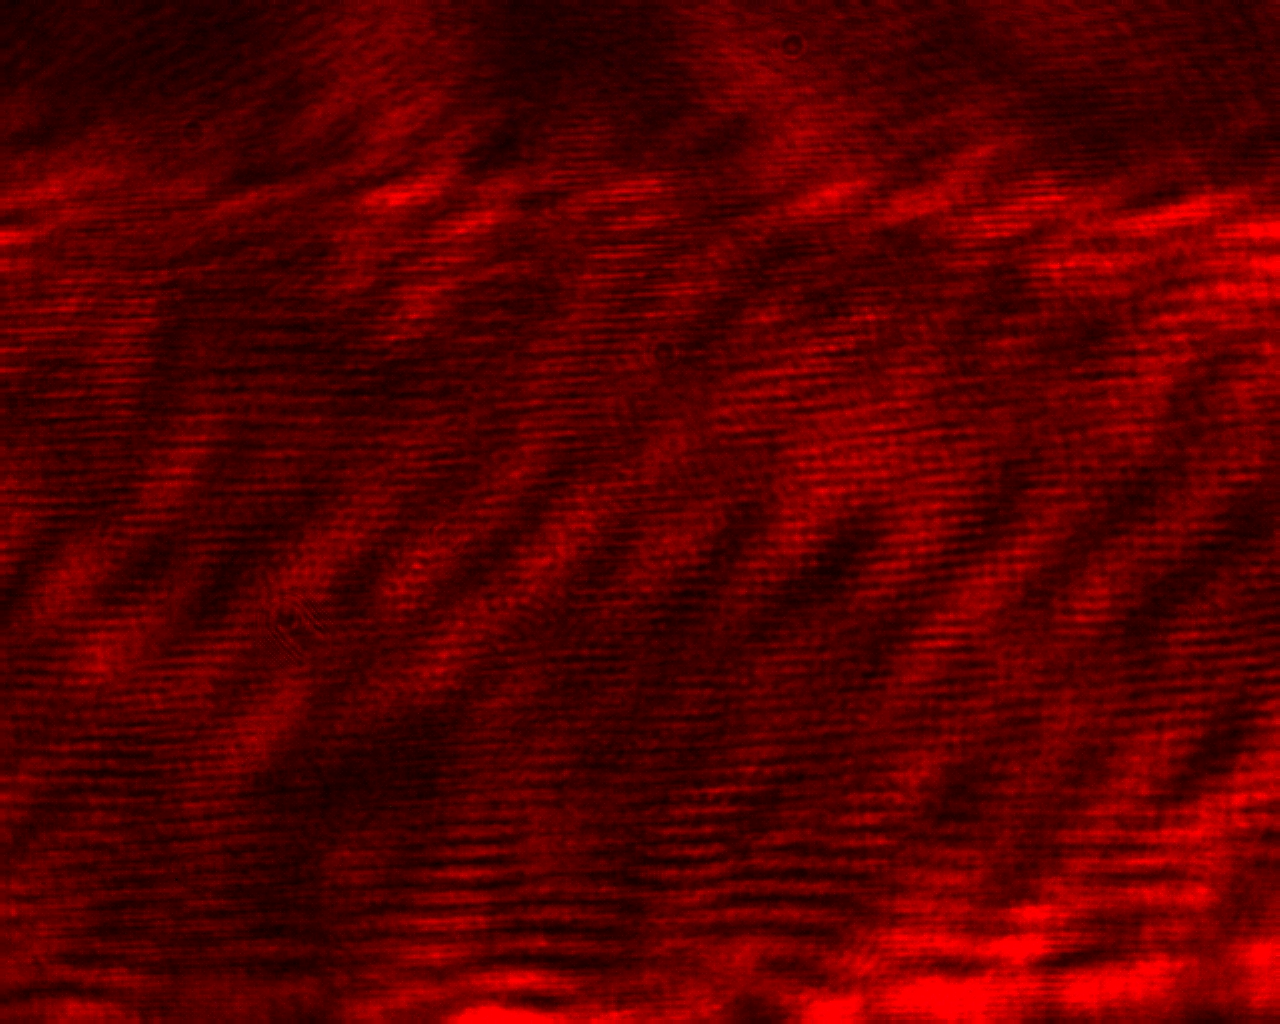
\includegraphics[width=\textwidth]{Pic_20260525203201995.png}
        \caption*{(f)}
    \end{minipage}
    \caption{实验记录图像（二）}
    \label{fig:records2}
\end{figure}

从图像记录可以看出，干涉图样不是在整个光斑范围内都保持相同清晰度。部分区域中亮暗条纹较集中、可见度较高，而远离该区域后条纹逐渐变弱，背景中散斑与光强起伏对条纹的影响更明显。该现象说明本实验光场具有有限空间相干尺度，只有互相对应的两点具有足够高空间相干性时，叠加后才能形成可观察的干涉条纹。

毛玻璃静止时，散斑结构对局部光强有明显调制，散斑内部仍可能出现条纹；毛玻璃旋转后，随机散斑在 CCD 曝光时间内被时间平均，不具有固定相位关系的部分被削弱，而空间相干性较强的区域仍保留可见条纹。因此，旋转毛玻璃条件下的图像更能体现部分相干光的横向相干范围。

\section{数据处理与分析}
\subsection{图像强度提取方法}
CCD 图像为红色干涉图像，因此取 RGB 图像的红色通道灰度值作为相对光强 $I$。对每幅图像先用亮度阈值确定有效光斑区域，再取有效光斑中部水平带作为分析区域。分析区域的纵向范围记为 $y_0\sim y_1$，横向范围记为 $x_0\sim x_1$。在该区域内沿 $y$ 方向求平均，得到横向一维平均强度剖面
\begin{equation}
    I(x)=\frac{1}{y_1-y_0}\sum_{y=y_0}^{y_1}I(x,y).
\end{equation}
为减小孤立亮点和暗背景像素对结果的影响，对 $I(x)$ 作平滑处理，并在宽度为 $\SI{120}{pixel}$、步长为 $\SI{20}{pixel}$ 的滑动窗口内取强度的 $90\%$ 分位数和 $10\%$ 分位数分别作为局部 $I_{\max}$ 与 $I_{\min}$，代入式~\eqref{eq:visibility} 计算局部条纹可见度 $V(x)$。

图~\ref{fig:roi-selection} 给出了各图像中实际用于提取强度剖面的区域。图~\ref{fig:visibility-profiles} 为由图像提取得到的局部条纹可见度随横向像素位置的变化。

\begin{figure}[htbp]
    \centering
    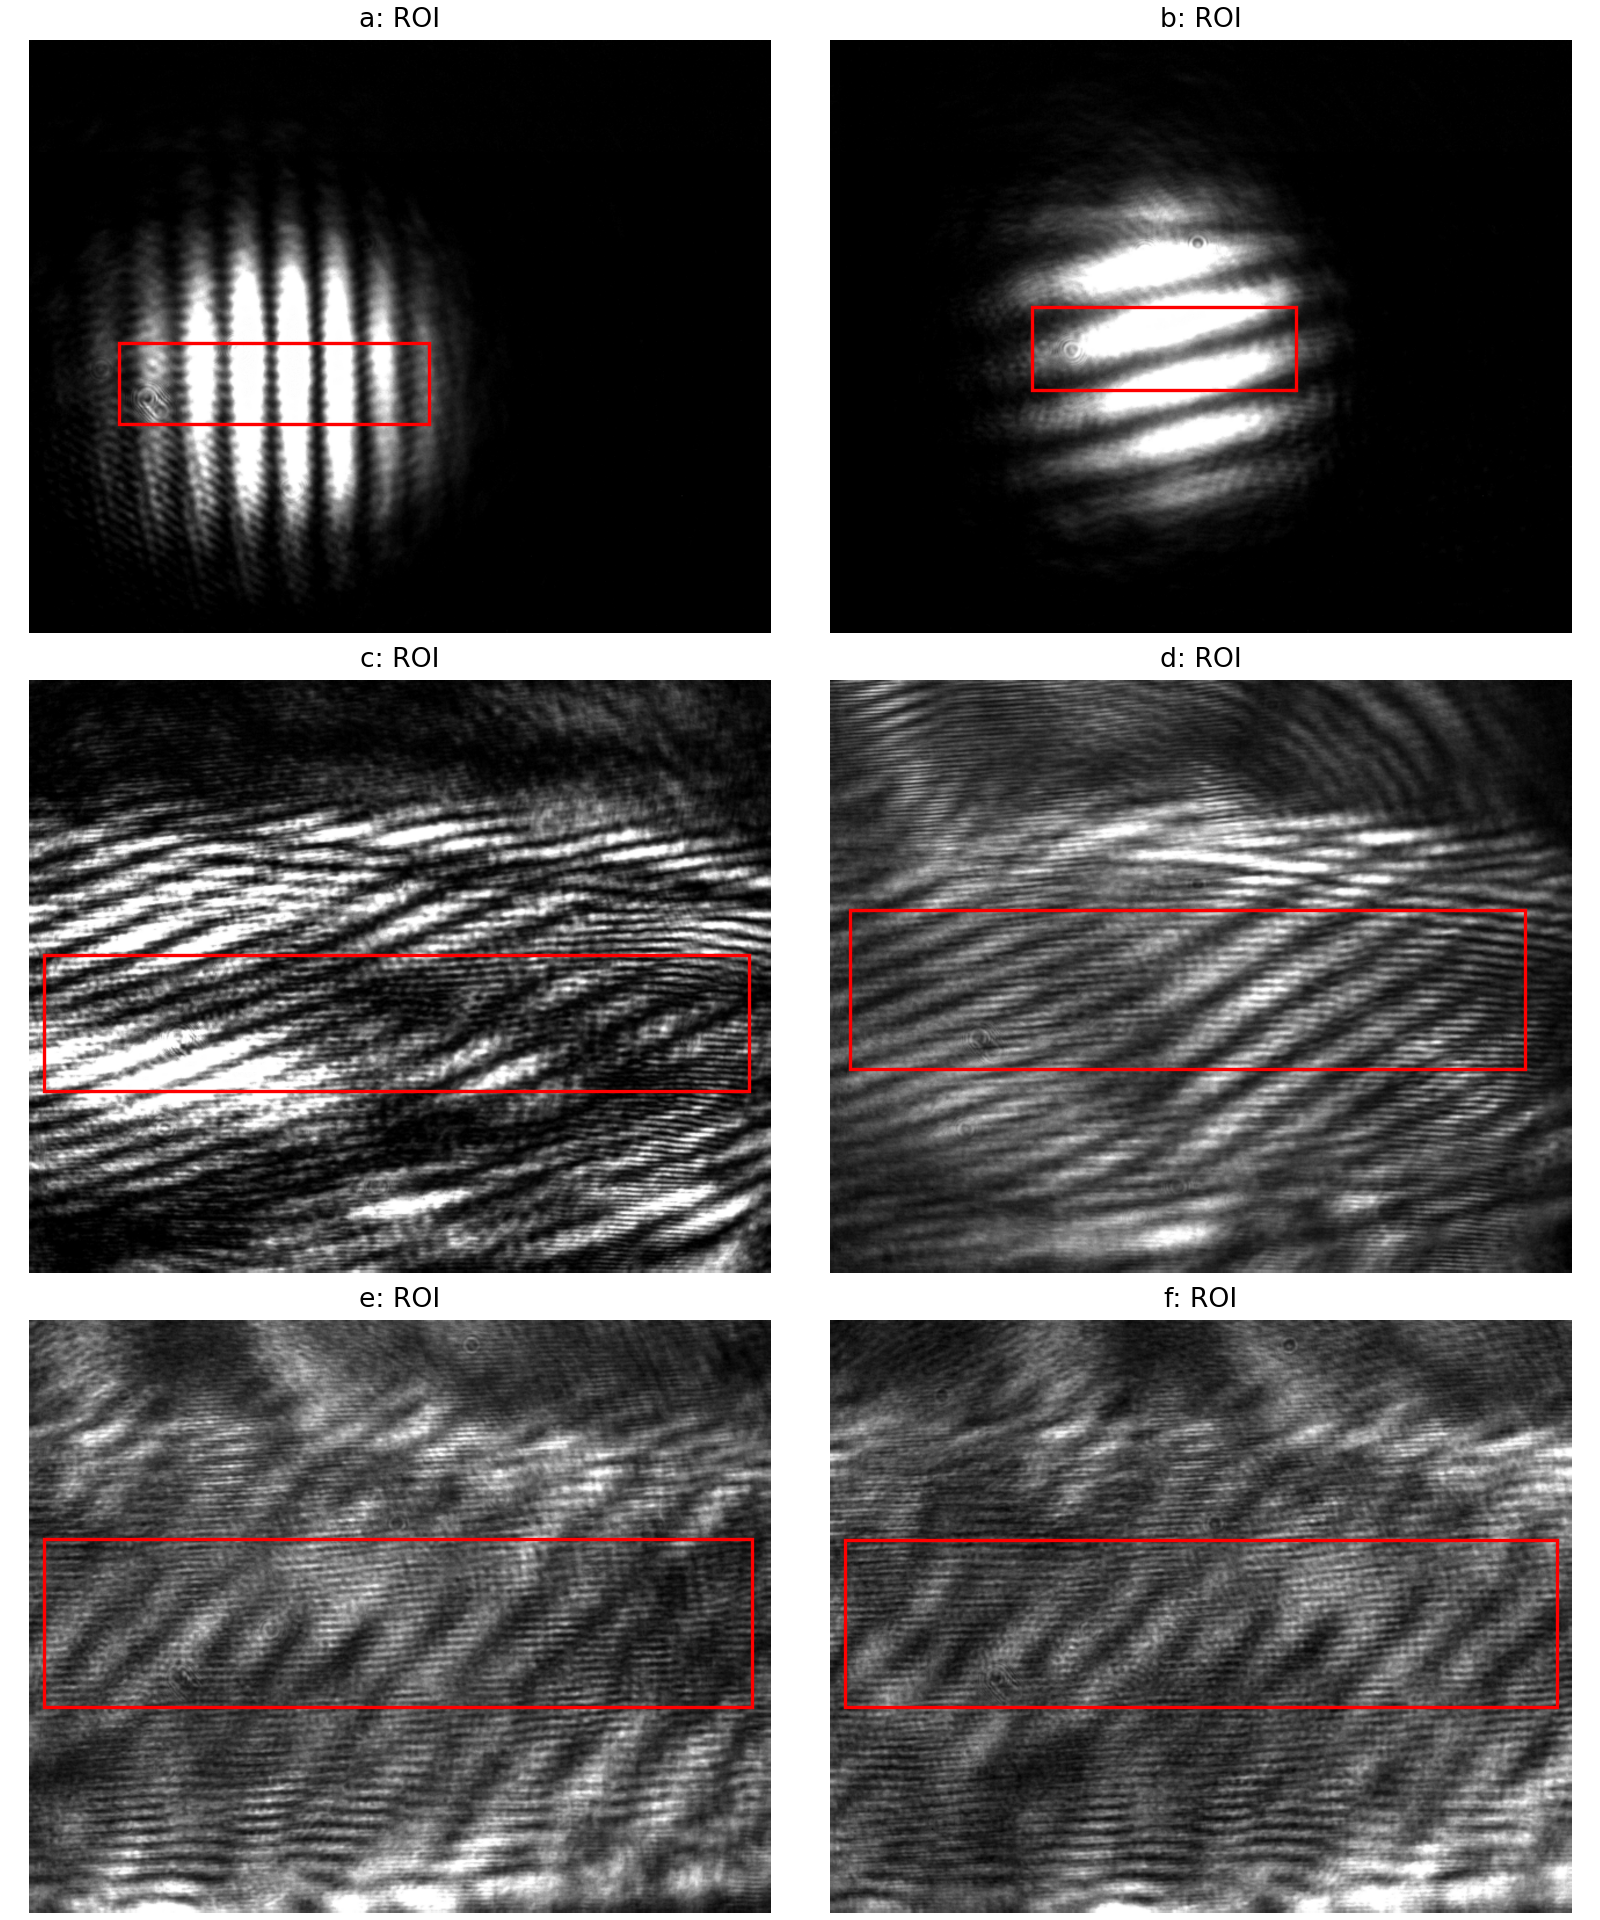
\includegraphics[width=0.86\textwidth]{roi_selection.png}
    \caption{CCD 图像中用于提取条纹强度剖面的分析区域}
    \label{fig:roi-selection}
\end{figure}

\begin{figure}[htbp]
    \centering
    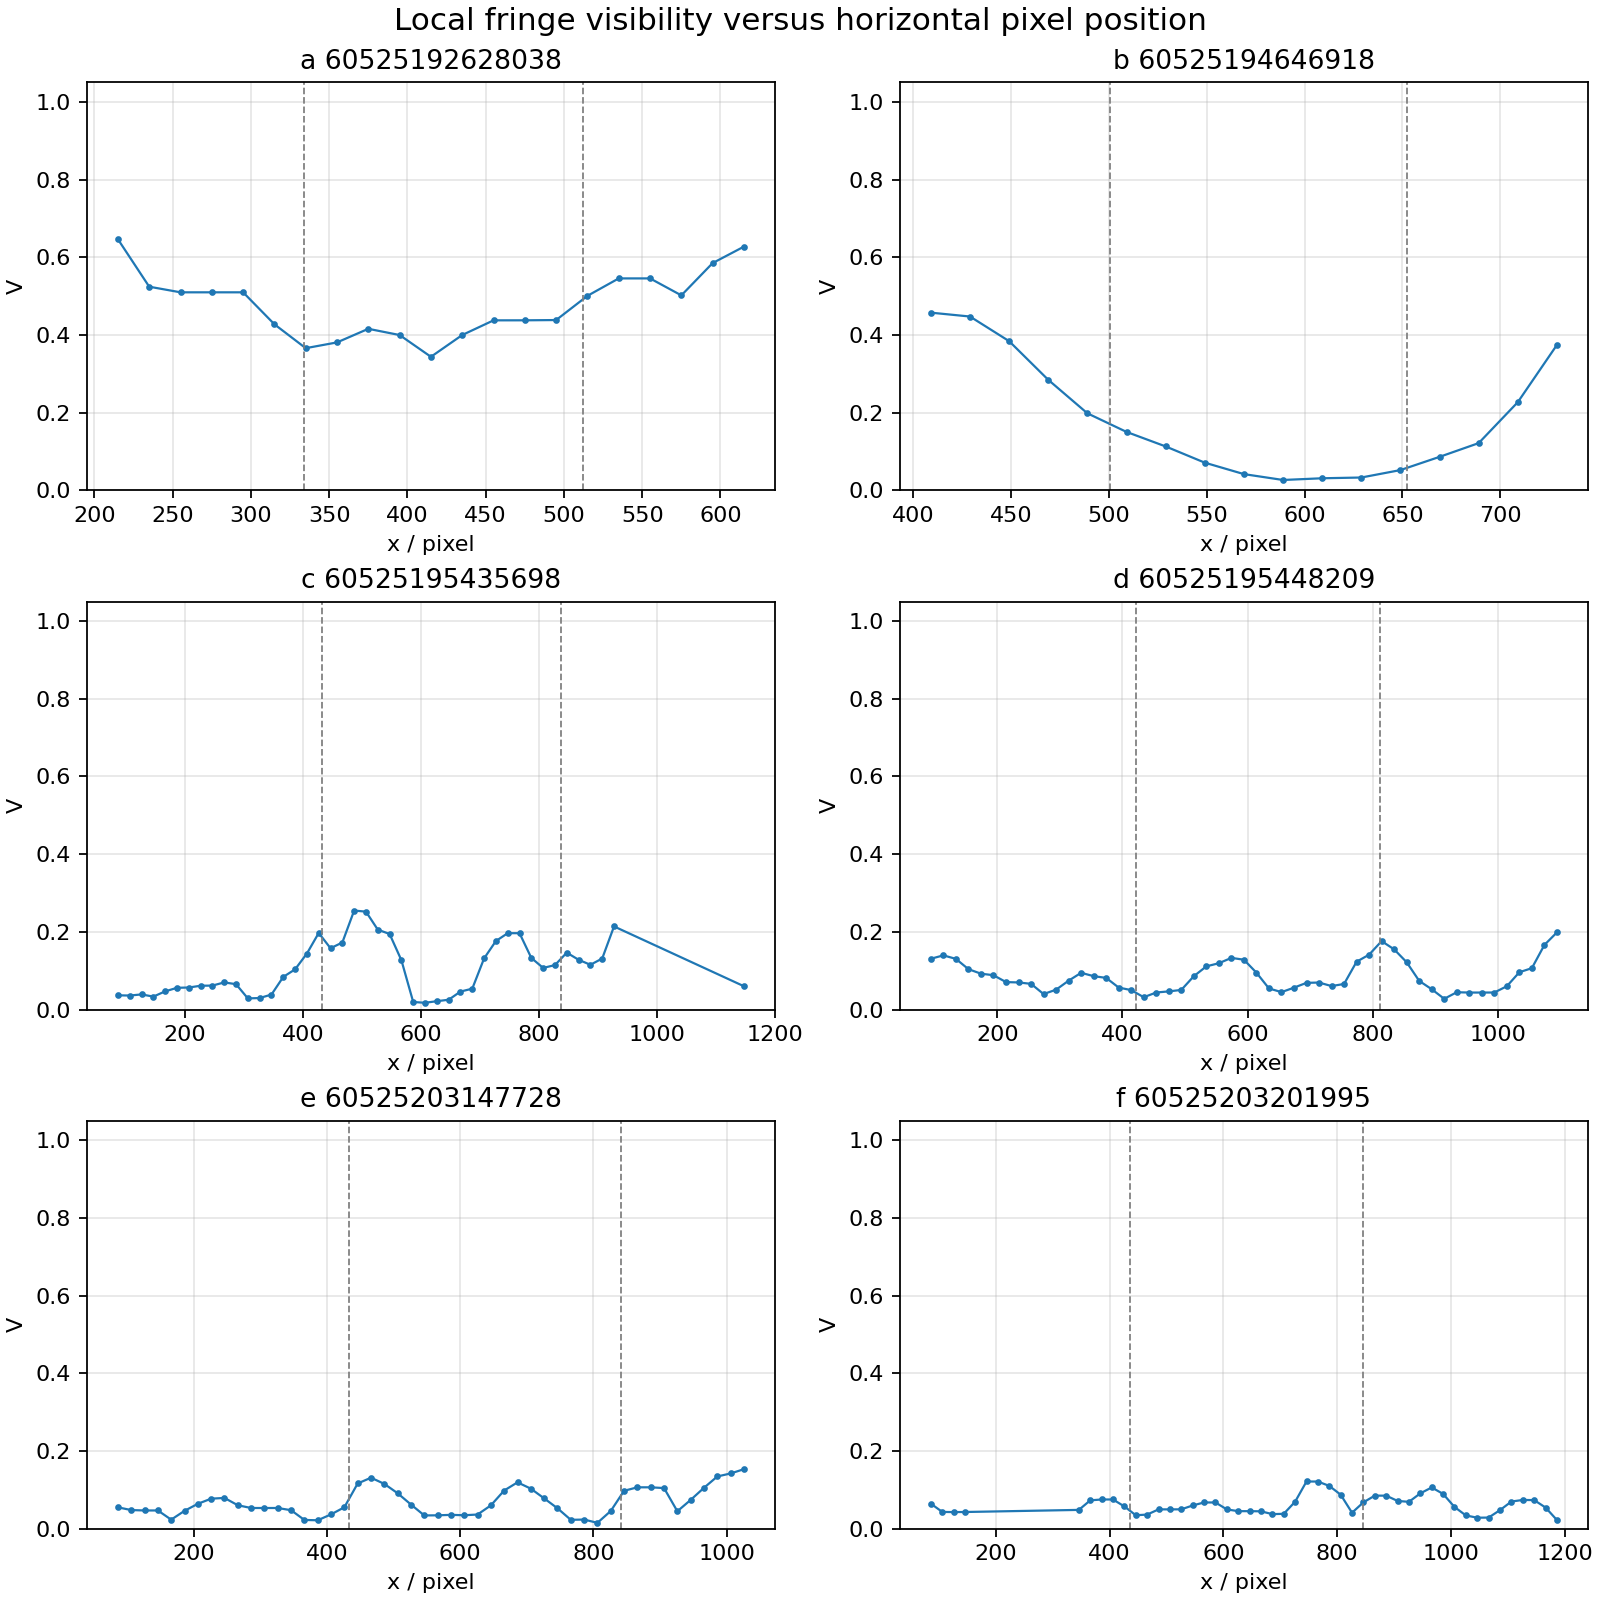
\includegraphics[width=0.88\textwidth]{visibility_profiles.png}
    \caption{由实验图像提取的局部条纹可见度 $V(x)$}
    \label{fig:visibility-profiles}
\end{figure}

\subsection{局部条纹可见度计算结果}
将每幅图像的横向分析范围三等分，分别计算左区、中区、右区的平均可见度，同时记录局部最大可见度 $V_{\max}$ 及其所在横向像素位置，结果见表~\ref{tab:visibility-results}。

\begin{table}[htbp]
    \centering
    \caption{图像提取得到的条纹可见度结果}
    \label{tab:visibility-results}
    \begin{tabular}{cccccccc}
        \toprule
        图像 & $x$ 范围/pixel & $y$ 范围/pixel & $\bar V_{\mathrm{L}}$ & $\bar V_{\mathrm{M}}$ & $\bar V_{\mathrm{R}}$ & $V_{\max}$ & $x(V_{\max})$/pixel \\
        \midrule
        (a) & 155--691 & 523--663 & 0.521 & 0.402 & 0.551 & 0.646 & 215 \\
        (b) & 349--804 & 460--604 & 0.354 & 0.065 & 0.202 & 0.457 & 409 \\
        (c) & 27--1243 & 474--708 & 0.066 & 0.130 & 0.133 & 0.255 & 487 \\
        (d) & 34--1199 & 397--671 & 0.084 & 0.081 & 0.094 & 0.199 & 1094 \\
        (e) & 26--1248 & 378--668 & 0.050 & 0.066 & 0.107 & 0.154 & 1026 \\
        (f) & 26--1255 & 379--667 & 0.058 & 0.062 & 0.065 & 0.122 & 746 \\
        \bottomrule
    \end{tabular}
\end{table}

从表~\ref{tab:visibility-results} 可见，图像 (a)、(b) 的局部最大可见度分别达到 0.646 和 0.457，说明其分析区域内存在较清晰的条纹；图像 (c)--(f) 的最大可见度降至 0.255、0.199、0.154 和 0.122，条纹对比度明显降低，图像中散斑和光强起伏占主要成分。该结果与直接观察图像得到的现象一致：部分实验条件下干涉条纹较清楚，而另一些条件下条纹被显著削弱。

图像 (a) 的较高可见度区域出现在 $x\approx215$ pixel 附近；图像 (b) 的较高可见度区域出现在 $x\approx409$ pixel 附近。二者最大值位置相差约 $194$ pixel，表明改变毛玻璃状态或位置后，满足较强空间相干条件的区域发生了明显横向移动。图像 (c)--(f) 的可见度整体较低，其中图像 (d)、(e) 的局部最大值位于右侧区域，而图像 (f) 的局部最大值位于中部偏右区域，说明在这些记录条件下只有较小范围内仍保留较弱条纹。

\subsection{不同区域条纹对比度差异}
实验图像中，条纹并非均匀分布在整个重叠光斑中。由表~\ref{tab:visibility-results} 可知，各图像左、中、右三个区域的平均可见度不同。例如图像 (a) 的左区和右区平均可见度分别为 0.521 和 0.551，均高于中区的 0.402；图像 (b) 的左区平均可见度为 0.354，明显高于中区的 0.065。图像 (d)--(f) 的三个区域平均可见度均低于 0.11，说明条纹只以较弱形式存在。

这种区域差异与柱透镜反转后的几何对应关系一致：CCD 上同一点处叠加的两束光来自源面上一对互为镜像的点，离相干性较好的对应区域越远，两点间横向距离越大。由式~\eqref{eq:coherence} 可知，空间相干度随横向距离快速衰减，所以远离相干性较好的区域时，条纹可见度降低。

\subsection{毛玻璃位置对条纹范围的影响}
改变毛玻璃位置会改变部分相干光源的等效源面位置及其经透镜后的成像关系，进而改变 CCD 平面上两束干涉光对应源面点的横向间距分布。图像 (a) 与 (b) 的 $V_{\max}$ 位置分别位于 $x=215$ pixel 与 $x=409$ pixel，明显条纹区域的位置发生横向移动；图像 (c)--(f) 中 $V_{\max}$ 下降到 0.26 以下，表明相应条件下有效相干区域明显缩小或条纹对比度整体下降。因此，图像数据支持“毛玻璃位于不同位置时条纹出现区域会变化”的判断。

\section{误差来源与改进}
\begin{enumerate}
    \item 光路调节误差：两臂光程差和平面镜相对倾角的微小偏差会改变条纹间距和方向，进而影响局部条纹可见度判断。
    \item 光学元件共轴误差：透镜、光阑、分束器、柱透镜与 CCD 若未严格共轴，会使两束光斑重叠区域减小或偏移。
    \item 毛玻璃转动状态：转速不足或不稳定时，CCD 曝光时间内的散斑平均不充分，部分随机散斑会残留在图像中。
    \item CCD 成像影响：曝光时间、增益设置和像素饱和会改变记录到的明暗强度，从而影响由图像估计的对比度。
\end{enumerate}

改进时可保持固定曝光和增益参数，沿垂直于条纹方向提取多条强度剖面，在相同窗口大小下计算局部可见度，并绘制可见度随横向位置的变化曲线，从而更定量地分析部分相干光的空间相干尺度。

\section{实验结论}
\begin{enumerate}
    \item 利用激光与旋转毛玻璃可以产生具有有限空间相干尺度的部分相干光源。
    \item 在改进迈克尔逊干涉光路中，柱透镜使其中一路光束发生竖直方向反转，使 CCD 上不同位置处叠加的两束光对应源面上不同横向间距的两点。
    \item 由图像提取的局部条纹可见度显示，图像 (a)、(b) 的最大可见度分别为 0.646 和 0.457，而图像 (c)--(f) 的最大可见度不超过 0.255，说明不同实验条件下条纹对比度差异显著。
    \item 图像 (a)、(b) 的最大可见度位置分别为 $x=215$ pixel 和 $x=409$ pixel，说明毛玻璃位置或状态改变会改变相干性较好区域在 CCD 平面上的位置。
\end{enumerate}

\section{思考题}
\textbf{毛玻璃位于不同位置时为什么条纹出现区域有变化？}

毛玻璃的位置决定了部分相干光源的等效源面位置、光束会聚或发散状态，以及源面横向坐标到 CCD 平面的映射关系。实验中柱透镜和反射镜使两束参与干涉的光近似互为镜像，CCD 上某一点处叠加的两束光对应于源面上一对横向分离的点。只有这对点的横向距离小于或接近相干性衰减尺度时，局部空间相干度才足够高，条纹才清晰可见。

当毛玻璃移动到不同位置时，透镜系统对等效源面的成像关系随之改变，CCD 上各位置对应的源面点对也发生改变。于是，满足较小横向间距、较高空间相干度的区域会移动、扩大或缩小，表现为干涉条纹出现区域发生变化。

\end{document}
